
\subsubsection{Pipeline}

En el proceso de Pull Request, tal y como se diseño~\nameref{par:testing}, se ejecuta el pipeline diseñado para garantizar la entrega de software testeado y con el estandar de calidad requerido.
Podemos ver en la figura~\cref{fig:githubActions} que los pasos son:

\begin{itemize}
    \item ejecutar los tests
    \item pasar el chequeo de estandar del código
    \item compilar en modo producción
\end{itemize}

faltarían el CD o continous delivery que ejecutaría los pasos de subir dicho ejecutable a un servidor, al menos para el programa manager.

\begin{figure}[H]
    \centering
    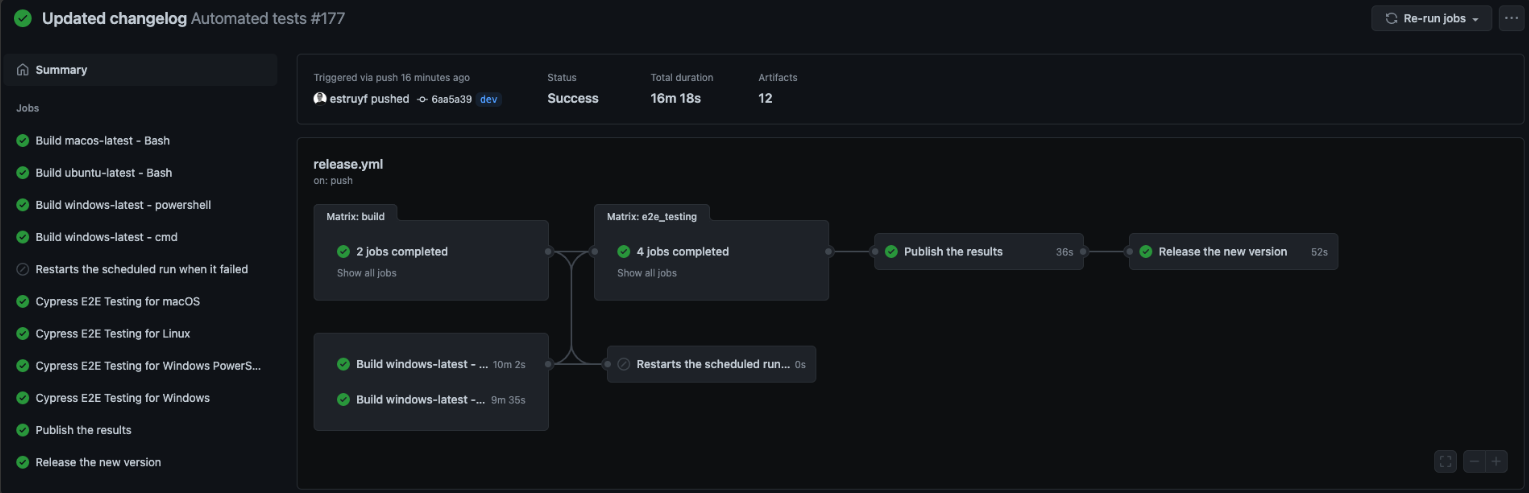
\includegraphics[height=0.2\textheight]{./part/Ejecucion/Seguimiento/PuestaAPunto/img/githubPipelines}
    \caption{Pipeline en Github}\label{fig:githubActions}
\end{figure}

\subsubsection{Montaje de prueba}

Para la prueba conjunta del sistema se ha desplegado un montaje como se ve en la figura~\cref{fig:Control-Diagrama UML de despliegue}

\begin{figure}[H]
    \centering
    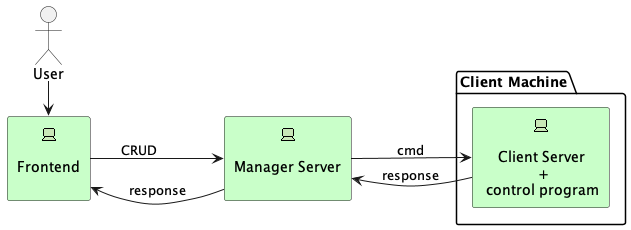
\includegraphics[height=0.2\textheight]{./part/Ejecucion/Seguimiento/PuestaAPunto/img/deploy}
    \caption{Diagrama de despliegue de prueba}\label{fig:despliegue de prueba}
\end{figure}

La imagen~\cref{fig:montaje en protoboard} muestra el montaje físico de conexión entre el el servidor cliente.
La Raspberry se conecta en una protoboard donde se realiza la conexión con el puente H y el motor de corriente continua.

\begin{figure}[H]
    \centering
    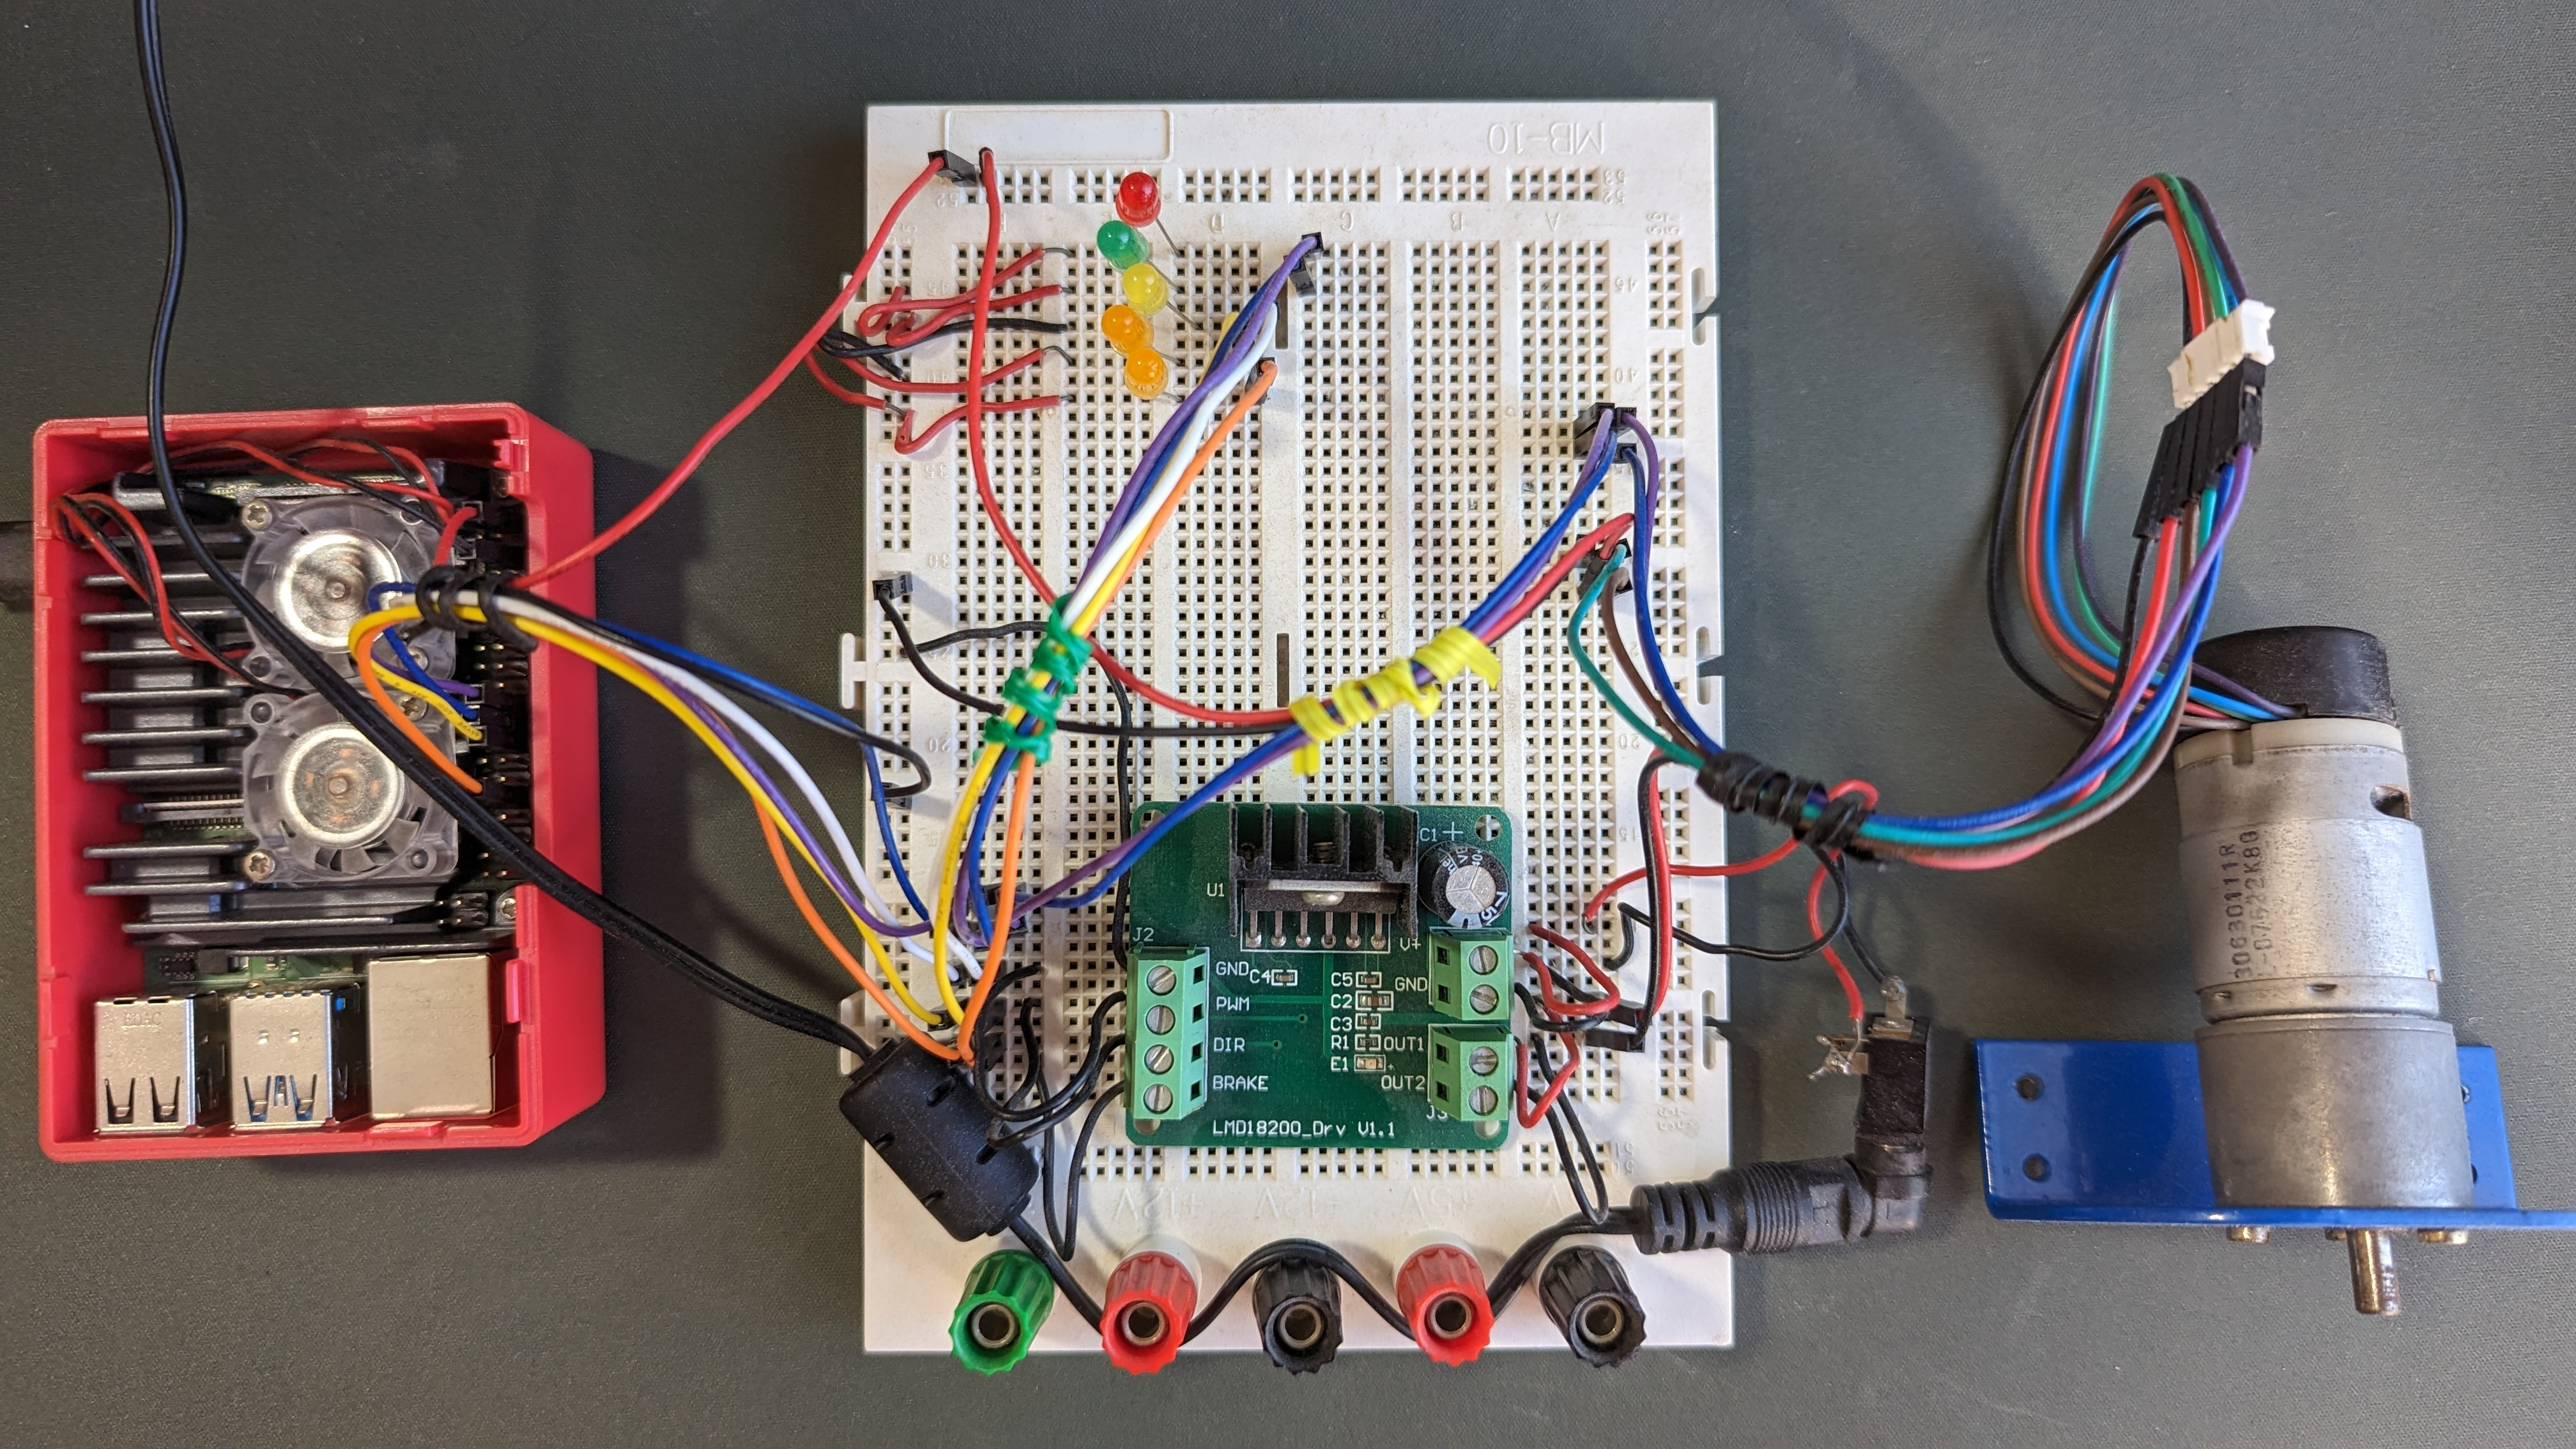
\includegraphics[height=0.2\textheight]{./part/Ejecucion/Seguimiento/PuestaAPunto/img/montajeProtoboard}
    \caption{Montaje en protoboard}\label{fig:montaje en protoboard}
\end{figure}

\subsubsection{Interfaz gráfica}

Para controlar el programa manager se ha desarrollado como añadido una interfaz gráfica.
En la figura~\cref{fig:frontend} podemos ver el listado de las tareas creadas, el estado en el que se encuentran y un boton para ejecutar manualmente las que son manuales.
Para ejecutar manualmente una tarea disponimos de una gráfica para ver en tiempo real la evolución de la variable controlada tal y como podemos ver en el~\cref{fig:runner}

\begin{figure}[H]
    \centering
    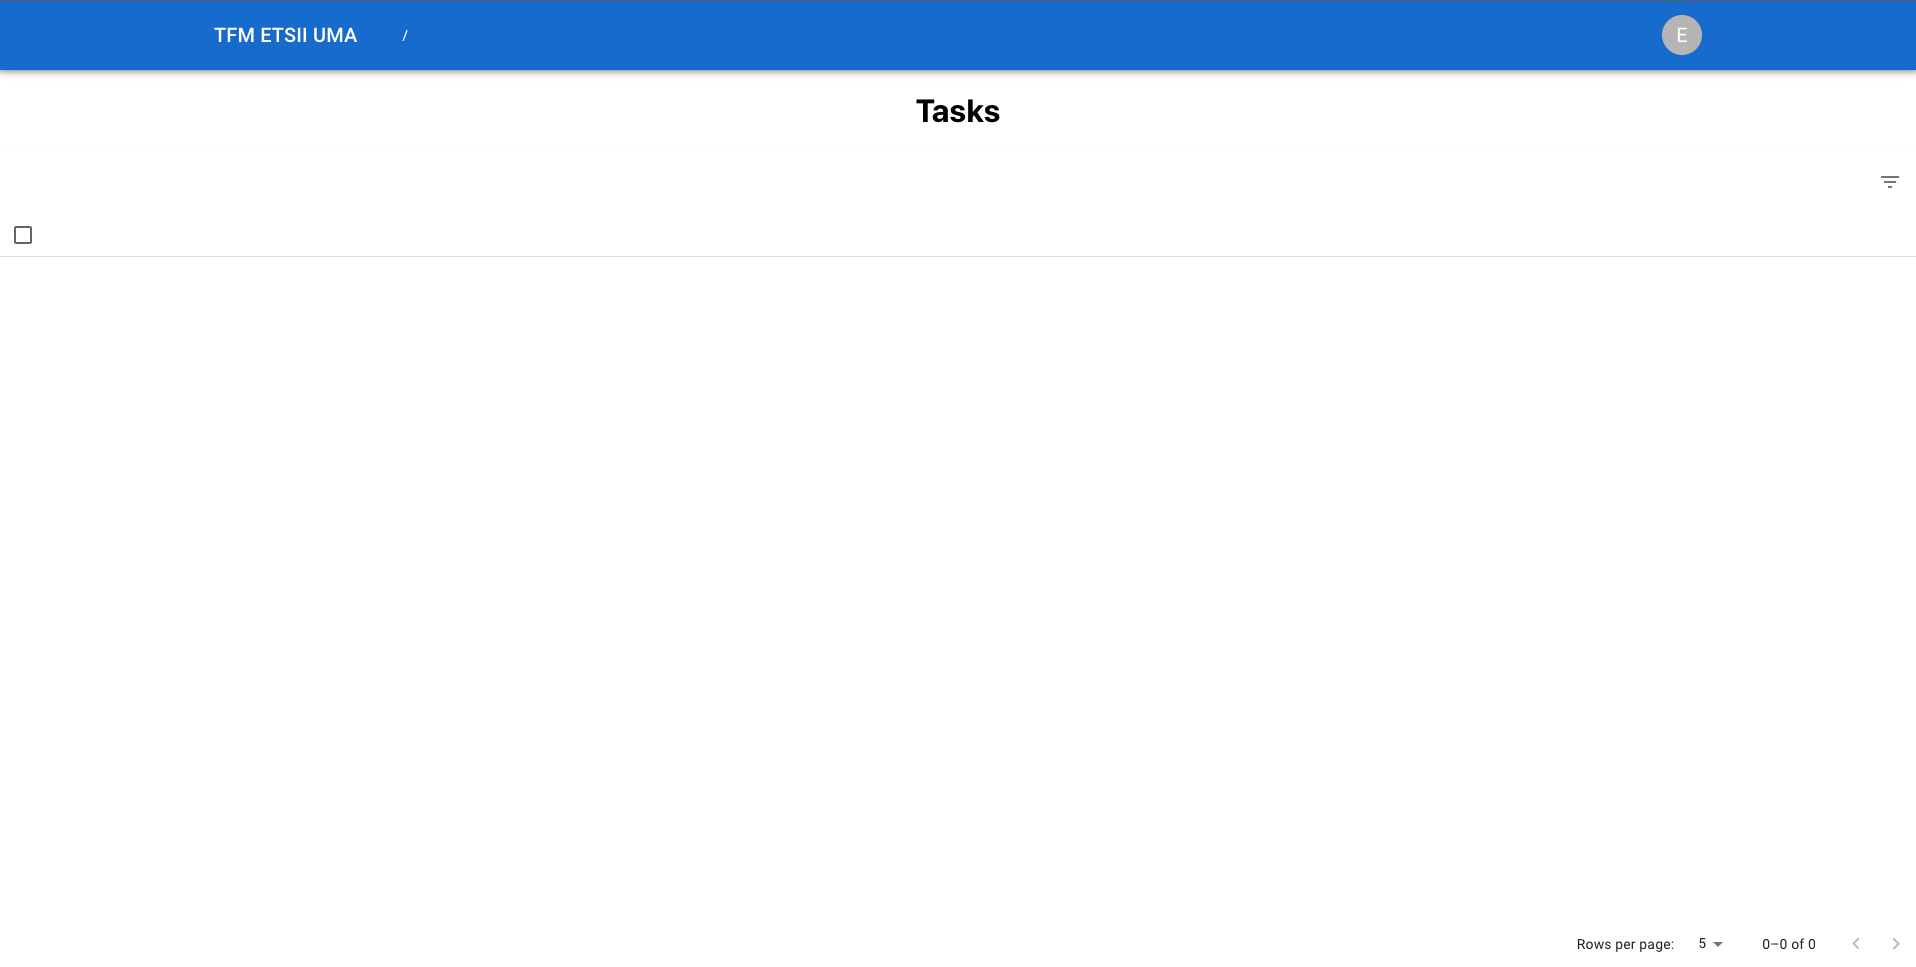
\includegraphics[height=0.2\textheight]{./part/Ejecucion/Seguimiento/PuestaAPunto/img/frontend}
    \caption{Frontend: task list}\label{fig:frontend}
\end{figure}

\begin{figure}[H]
    \centering
    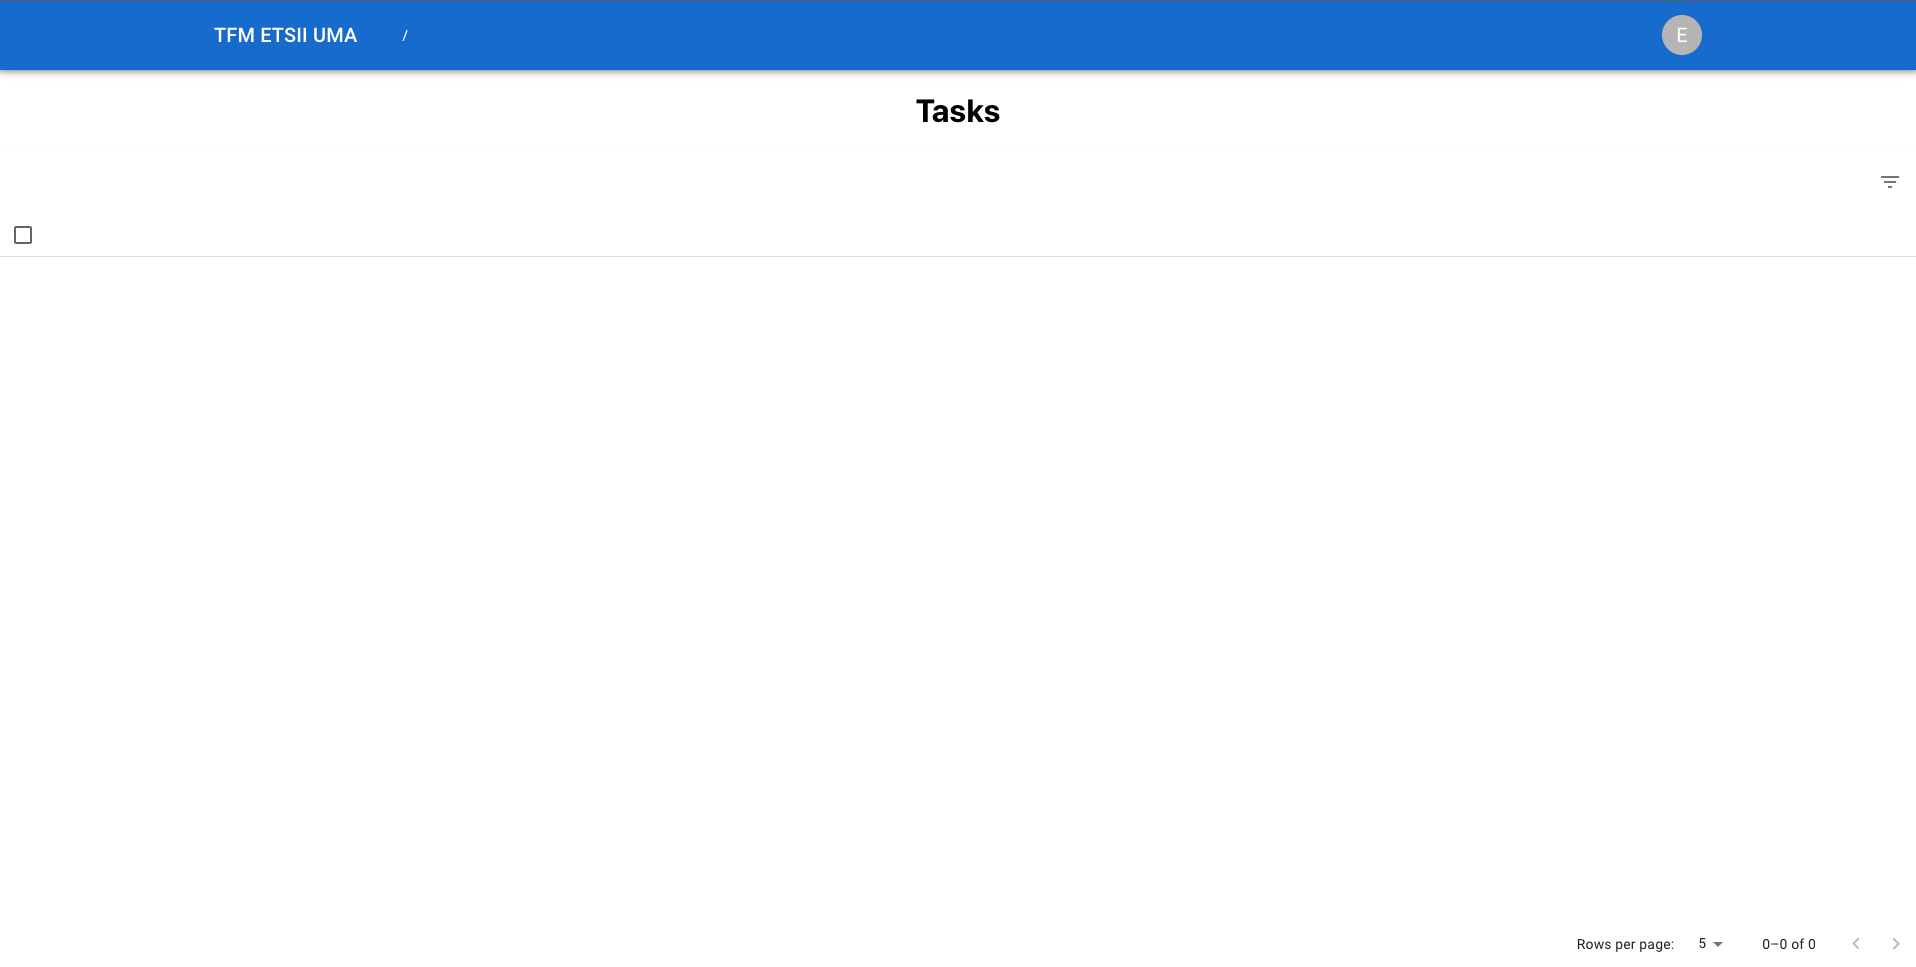
\includegraphics[height=0.2\textheight]{./part/Ejecucion/Seguimiento/PuestaAPunto/img/runner}
    \caption{Frontend: runner}\label{fig:runner}
\end{figure}